\chapter*{Print NPM menggunakan pembagian npm dengan mod 3}
\par karna hasil bagi dengan mod 3 sama dengan 0 maka menggunakan bintang(*)
\begin{enumerate}
   

\item buka spyder dan ketikan kode seperti berikut
	\begin{figure} [h]
	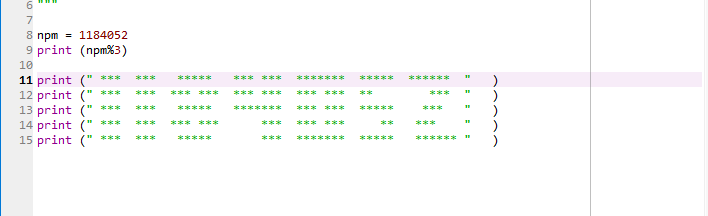
\includegraphics[width=7cm]{npm/npm13.png}
	\centering
	\end{figure}
	
	
	
 \item maka akan tercetak 
 \begin{figure} [h]
	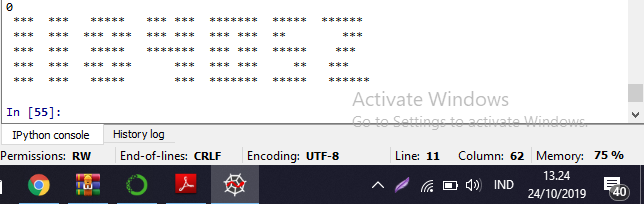
\includegraphics[width=7cm]{npm/npm14.png}
	\centering
	\end{figure}
 
	
	\end{enumerate}